\begin{figure}[H]
    \centering
    % 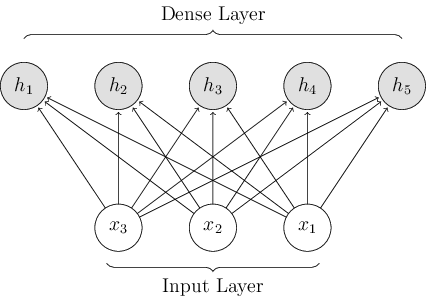
\includegraphics[width=.5\linewidth]{mainmatter/3-Methodology/images/dense.png}
    % \captionsetup{justification=centering,margin=0cm}

\begin{tikzpicture}[->,>=stealth',shorten >=1pt,auto,node distance=2.8cm,
    semithick]

      \tikzstyle{every state}=[text=black]
      \node[state]          (A)   {$h_1$};
      \node[state]         (B)  [right of=A] {$h_2$};
      \node[label=above:{Dense Layer},state]         (C) [right of=B] {$h_3$} ;
      \node[state]         (D) [right of=C] {$h_4$};
      \node[state]         (E) [right of=D] {$h_5$};

      \node[state]         (X1) [below of=B] {$x_3$};
      \node[state, label=below:{Input Layer}]         (X2) [right of=X1]       {$x_2$};
      \node[state]         (X3) [right of=X2]       {$x_1$};

      \path (X1) 
      edge              node {} (A)
      edge              node {} (B)
      edge              node {} (C)
      edge              node {} (D)
      edge              node {} (E)
      % edge              node {1,1,R} (C)
      (X2) 
      edge              node {} (A)
      edge              node {} (B)
      edge              node {} (C)
      edge              node {} (D)
      edge              node {} (E)
      % edge              node {0,1,L} (C)
      (X3)
      edge              node {} (A)
      edge              node {} (B)
      edge              node {} (C)
      edge              node {} (D)
      edge              node {} (E);
      % edge [bend left]  node {1,0,R} (E);

\end{tikzpicture}

  
\caption[Dense Layer]{The input nodes are represented by \textit{x} and the weights \textit{h} are applied to each values of input nodes to generate an output. The output is the blended value of input activations with the model's weight functions}
\label{fig:dense}
\end{figure}
